%\documentclass[11pt,a4paper]{article}
\documentclass[11pt,a4paper]{scrartcl}
%\documentclass[11pt,a4paper,oneside]{book}
\usepackage[british,UKenglish,USenglish,english,american]{babel}
%\usepackage[a4paper, total={16cm, 23cm}]{geometry}
\usepackage[tmargin = 1.25in,bmargin = 1.25in,lmargin = 0.75in,rmargin = 0.75in]{geometry}
\usepackage{tikz}
\usepackage{graphicx}
\usepackage{pgfplots}
\pgfplotsset{width=12cm,compat=1.9}
\usepackage{setspace}
\usepackage{chemmacros}
\usepackage{chemfig}
%\usepackage{ghsystem}
%\usechemmodule{redox}
%\usepackage{chemnum}
%\usepackage{bohr}
%\usepackage{elements}
%\usepackage{endiagram}
%\usepackage{modiagram}
%\usepackage{chemgreek}
%\usepackage{mhchem}
\usepackage{esint}
\usepackage{tabularray}

\usepackage{makeidx}
\usepackage{epstopdf}

\usepackage{amssymb}
\usepackage{mathrsfs}
%\usepackage{minted}
\usepackage{bm}
\usepackage{amsmath}
\usepackage{enumitem}
\usepackage[english]{varioref}
\usepackage[english]{babel}
\usepackage{lipsum}
\usepackage{fancyhdr}
\pagestyle{fancy} 
\usepackage{float}
\usepackage{empheq}
\usepackage[framemethod=tikz]{mdframed}
\usepackage{epstopdf}
\numberwithin{equation}{section}
\usepackage{eso-pic}
\usepackage{calc}
\usepackage{nccmath}
\usepackage{caption}
\usepackage{subcaption}
\usepackage{gensymb}
\usepackage{amsfonts,amsthm,epsfig,epstopdf,titling,url,array}
\usepackage{siunitx}
\sisetup{input-digits = 0123456789\pi}
\usepackage[symbol]{footmisc}
\usepackage{xcolor}
\usepackage{multicol}
\usepackage{boondox-cal}
\DeclareSIUnit\atm{atm}
\setcounter{secnumdepth}{3}
\setcounter{tocdepth}{3}
\usepackage{booktabs}
\usepackage{blindtext}
\usepackage{changepage}
\usepackage{longtable}

% \usepackage{draftwatermark}
% \SetWatermarkText{DRAFT}
% \SetWatermarkScale{5}

\DeclareSIUnit\atm{atm}

\pagestyle{fancy} 
\fancypagestyle{firstpage}{
	\rhead{
	}
}
\fancyhead[L]{\small\slshape\nouppercase{\leftmark}}
\chead{}
\rhead{ 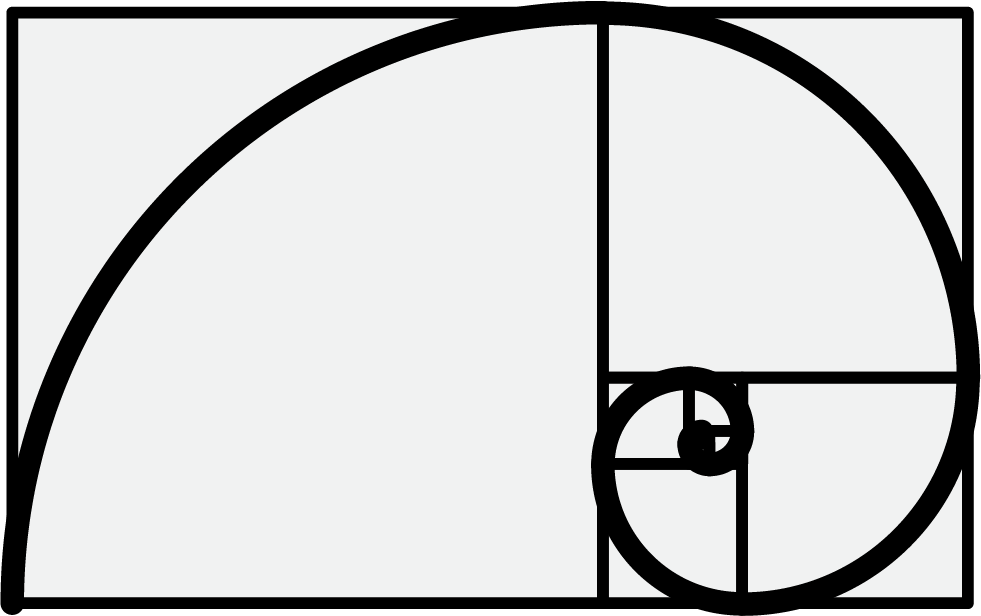
\includegraphics[height=0.75cm]{figures/pwr-control_logo_doc.png}
}
\lfoot{\textit{}}
\cfoot{-\ \thepage\ -}
\rfoot{\textit{}}

\DeclareMathOperator{\rank}{rank}
\DeclareMathOperator{\atantwo}{atan2}
\DeclareMathOperator{\arctantwo}{arctan2}
\DeclareMathOperator{\spn}{span}

\renewcommand{\headrulewidth}{0.4pt}
\renewcommand{\footrulewidth}{0.4pt}
\newcommand{\abs}[1]{\left|#1\right|}
\definecolor{mycolor1}{rgb}{0.97, 0.97, 0.97}
\definecolor{mycolor2}{rgb}{0.97, 0.97, 0.97}
\definecolor{tableShade}{gray}{0.9}
\newcommand{\sign}{\text{sign}}
\newcommand{\centered}[1]{\begin{tabular}{@{}l@{}} #1 \end{tabular}}
\theoremstyle{it}
\newtheorem{defn}{Definition}[section]
\newtheorem{assumption}{Assumption}[section]
\newtheorem{thm}{Theorem}[section]
\newtheorem{lemma}{Lemma}[section]
\newtheorem{corollary}{Corollary}[section]
\theoremstyle{definition}
%\theoremstyle{it}
\newtheorem{example}{Example}[section]
\let\eqrefn\eqref
\renewcommand{\eqref}[1]{Eq.~(\ref{#1})}

\newenvironment{myitemize_1}
{ \begin{itemize}[topsep=4pt]
		\setlength{\topsep}{2pt}		
		\setlength{\itemsep}{2pt}
		\setlength{\parskip}{2pt}
		\setlength{\parsep}{2pt}    }
	{ \end{itemize}                  	}

\newenvironment{myitemize_2}
{ \begin{itemize}[topsep=4pt]
		\setlength{\topsep}{2pt}		
		\setlength{\itemsep}{2pt}
		\setlength{\parskip}{2pt}
		\setlength{\parsep}{2pt}    }
	{ \end{itemize}   					}


\newmdenv[innerlinewidth=0.5pt, roundcorner=4pt,backgroundcolor=mycolor2, 
linecolor=mycolor1,innerleftmargin=6pt,
innerrightmargin=6pt,innertopmargin=6pt,innerbottommargin=6pt]{mybox}

\title{\textbf{ 
		\begin{LARGE}
			Extended Kalman Filter:
		\end{LARGE} \\[24pt]
		\begin{Large}
	Application to PSM with Ttype MPC Three Phase Inverter.
	\end{Large}}
}
\author{\textbf{Davide Bagnara}}

\begin{document}
	\thispagestyle{firstpage}
	\begin{mybox}
		\maketitle
		\vspace{125mm}
	\end{mybox}
	\newpage
	\tableofcontents
	\listoffigures	
	\listoftables
	\newpage
	
	{In this document the model of a generic flexible shaft is derived.}

\begin{onehalfspace}
\section{PMSM MPC with EKF}
\subsection{Introduction}
In this section we are going to develop a model predictive control (MPC) for a 
permanent magnet synchronous motor (PMSM) by the use of an observer based on 
the extended Kalman filter theory (EKF). 

The $\alpha\beta$ model representation of the PMSM is here reported
\begin{mybox}
	\textbf{PMSM Mathematical Model in Stationary Reference Frame}
	\begin{equation}\label{pmsm_problem_1_eq_1}
		\left\lbrace \begin{aligned}
			& \vec{u}_{\alpha\beta}(t)-\mathbf{R}^{\alpha\beta}\ 
			\vec{i}_{\alpha\beta}(t)-\mathbf{L}^{\alpha\beta}\ 
			\frac{d\vec{i}_{\alpha\beta}(t)}{dt}-\omega(t) \begin{bmatrix} 
				0 & -1 \\ 1 & 0\end{bmatrix} \vec{\psi}^r_{\alpha\beta} = 0 
			\\[6pt]
			& \frac{d\vec{\psi}^r_{\alpha\beta}(t)}{dt} = \omega(t) 
			\begin{bmatrix} 0 & -1 \\ 1 & 0\end{bmatrix} 
			\vec{\psi}^r_{\alpha\beta}(t) \qquad 
			\vec{\psi}^r_{\alpha\beta}(0) = \begin{bmatrix} \Psi^M &  0 
			\end{bmatrix}^T \\[6pt]
			& \frac{d}{dt}{\omega}_m(t) = 
			\frac{1}{J}\Bigg[\frac{3}{2}p\Big[\psi^r_{\alpha}(t)i_{\beta}(t)-\psi^r_{\beta}(t)i_{\alpha}(t)\Big]
			-\tau_l(t) -b{\omega}_m(t)\Bigg]
			\\[6pt]
			& \frac{d}{dt}{\theta}(t) = \omega(t) = p\omega_m(t)
		\end{aligned} \right. 
	\end{equation}
	or in a more explicit representation
	\begin{equation}\label{pmsm_problem_1_eq_2}
		\left\lbrace \begin{aligned}
			& \frac{d}{dt} i_\alpha(t)= -\frac{R_s}{L_\alpha}i_\alpha(t) 
			+\frac{\omega(t)}{L_\alpha}\psi_\beta(t)+\frac{1}{L_\alpha}u_\alpha(t)
			\\[6pt]
			& \frac{d}{dt} i_\beta(t)= -\frac{R_s}{L_\beta}i_\beta(t) 
			-\frac{\omega(t)}{L_\beta}\psi_\alpha(t)+\frac{1}{L_\beta}u_\beta(t)
			\\[6pt]
			&\frac{d}{dt} \psi_\alpha^r(t) = -\omega(t)\psi_\beta^r(t) \\[6pt]
			&\frac{d}{dt} \psi_\beta^r(t) = \omega(t)\psi_\alpha^r(t) \\[6pt]
			& \frac{d}{dt}{\omega}_m(t) = 
			\frac{1}{J}\Bigg[\frac{3}{2}p\Big[\psi^r_{\alpha}(t)i_{\beta}(t)-\psi^r_{\beta}(t)i_{\alpha}(t)\Big]
			-\tau_l(t) -b{\omega}_m(t)\Bigg]
			\\[6pt]
			& \frac{d}{dt}{\theta}(t) = \omega(t) = p\omega_m(t)
		\end{aligned} \right. 
	\end{equation}
	where $p$ is the number of poles pairs, $b$ the bearing viscosity and 
	$\tau_l(t)$ the external and unknown load (disturbance).
\end{mybox}

Remind also the following nomenclature
\begin{itemize}
	\item[--] $i_\alpha(t)$ - is the $\alpha$ component of the stator current.
	\item[--] $i_\beta(t)$ - is the $\beta$ component of the stator current.
	\item[--] $u_\alpha(t)$ - is the $\alpha$ component of the stator input voltage.
	\item[--] $u_\beta(t)$ - is the $\beta$ component of the stator input voltage.
	\item[--] $\psi_\alpha^r(t)$ - is the $\alpha$ component of the permanent magnet rotor flux linkage to the stator.
	\item[--] $\psi_\beta^r(t)$ - is the $\beta$ component of the permanent magnet rotor flux linkage to the stator.
	\item[--] $\omega_m(t)$ - is the mechanical rotor speed.
	\item[--] $\omega(t)$ - is the stator electrical pulsation related to the mechanical rotor speed by the relation $\omega(t)=p\omega_m(t)$.
	\item[--] $p$ - is the number of pole pairs of the rotor.
	\item[--] $\vartheta_m(t)$ - is the mechanical rotor position.
	\item[--] $\vartheta(t)$ - is the stator electrical phase related to the mechanical rotor position by the relation $\vartheta(t)=p\vartheta_m(t)$.
	\item[--] $\tau_m(t)$ is the electromagnetic torque generated by the PMSM
	\item[--] $\tau_l(t)$ is the external load and is unknown.
\end{itemize}

\subsection{Control design}
In order to design a proper control structure we summarize here the main working hypothesis which we are takein into account
\begin{itemize}
	\item[--] The PMSM is isotropic, that means $L_\alpha=L_\beta=L_s$.
	\item[--] The motor is driven by an inverter based on space vector 
	modulation.
	\item[--] The only stator current are available for the measure.
	\item[--] The time constant of the mechanic system is twenty times greater 
	than the time constant of the electrical and fluxes systems.
\end{itemize}

\textbf{The scope of the control design is to implement a rotor speed control with zero tracking error in steady state condition.}

\vspace{5mm}
As first draft we can draw the control architecture be made by the following substructures
\begin{itemize}
	\item[--] A speed control based on PI-control.
	\item[--] A substructure which convert the torque reference (as output of the speed control) into a set of current references $i_\alpha^{ref}$ and $i_\beta^{ref}$. Remind the motor is a three phase system and that means must be represented by two components. 	
	\item[--] A rotor flux vector estimator based on the Extended Kalman Filter.
	\item[--] A rotor speed estimator used to calculate $\hat{\omega}$ from $\hat{\vartheta}$ based on double integrator observer.
\end{itemize}
A schematic overview of the proposed control architecture is shown in 
Figure~\eqref{pmsmctrl_overview}
\begin{figure}[H]
	\centering
	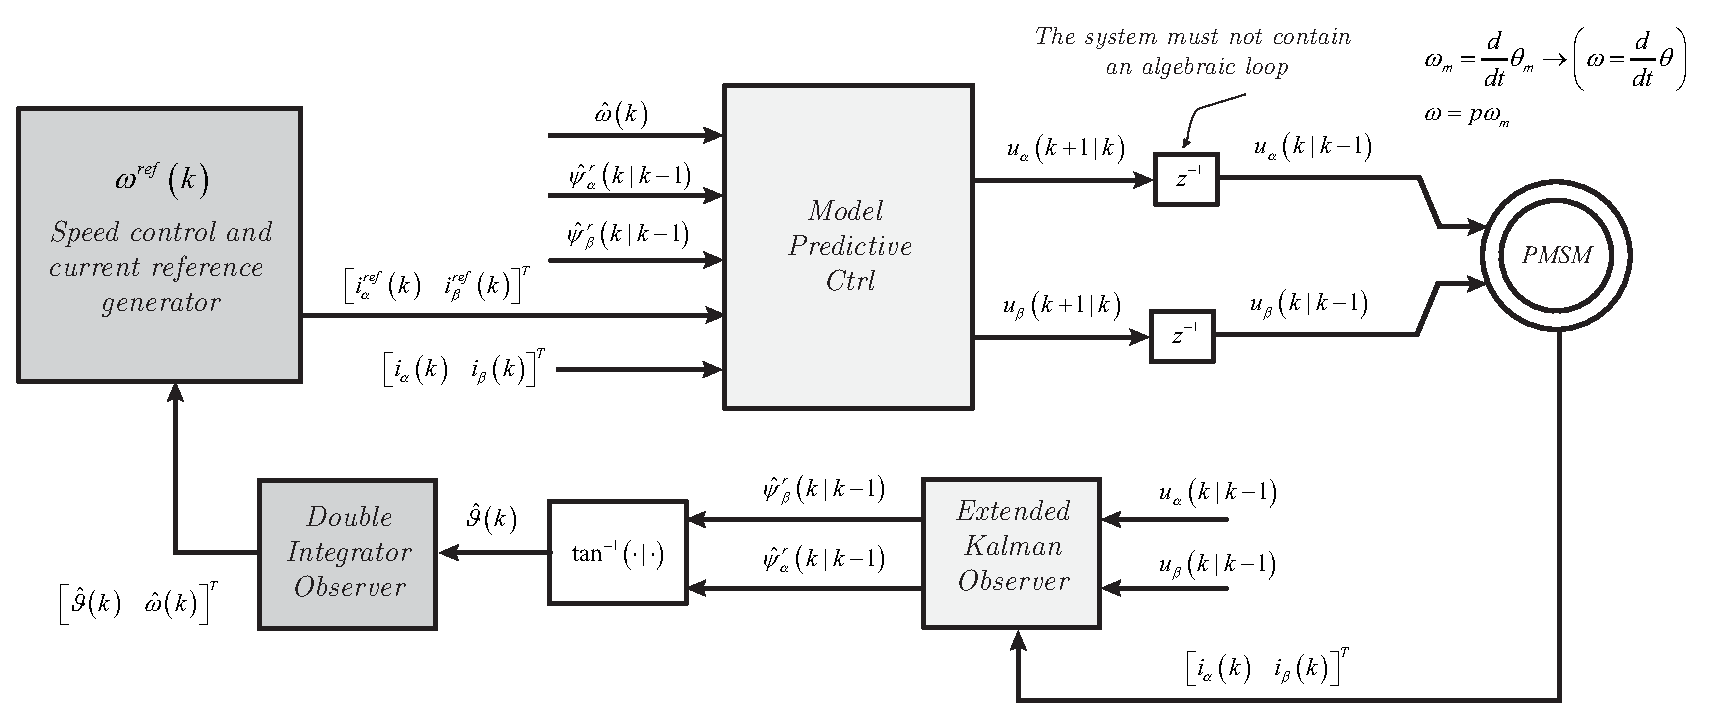
\includegraphics[width = 500pt, angle=0, 
	keepaspectratio]{figures/mpc/pmsm_ctrl_ab_2.eps}
	\captionsetup{width=.5\textwidth}
	\caption{PMSM control architecture.}
	\label{pmsmctrl_overview}
\end{figure}

In order to implement the selected control architecture the following 
mathematical substructures shall be investigated
\begin{itemize}
	\item[--] A discrete time representation of the mathematical model of the 
	PMSM.
	\item[--] The concept of the space vector and its correlation with an 
	IGBT-based Inverter.
	\item[--] A trajectory tracking cost function for the MTP. MPC is an 
	optimal control and needs a cost function to be used to derive the optimal 
	inverter output voltage.
	\item[--] Torque to current reference generator (the mechanical side 
	\textit{works} with torque but the electrical side \textit{works} with 
	currents).
	\item[--] A discrete time representation of the fluxes observer
	\item[--] A discrete time representation of the double integrator observer, see also Example~\ref{DoubleIntegratorObserver}.
\end{itemize}
\subsubsection{Model discretization}
As already mentioned, in order to implement our control structure a discrete-time representation 
of the system of Eq.~\eqref{pmsm_problem_1_eq_2} shall be derived. By the use of 
the Euler approximation for the derivatives using the sampling time $t_s$, that is 
\begin{equation}\label{pmsm_problem_1_eq_3}
	\frac{d}{dt}x(t)\approx\frac{x[(k+1)t_s]-x(kt_s)}{t_s}=\frac{x(k+1)-x(k)}{t_s}
\end{equation}
we obtain the following discrete time representation of the PMSM model
\begin{mybox}
	\textbf{Discrete-time representation of the PMSM}
	\begin{equation}\label{pmsm_problem_1_eq_4}
		\left\lbrace \begin{aligned}
			& i_\alpha(k+1)=\Big(1-t_s\frac{R_s}{L_\alpha}\Big) i_\alpha(k) 
			+t_s\frac{\omega(k)}{L_\alpha}\psi_\beta(k)+\frac{t_s}{L_\alpha}u_\alpha(k)
			\\[6pt]
			& i_\beta(k+1) = \Big(1-t_s\frac{R_s}{L_\beta}\Big)i_\beta(k) 
			-t_s\frac{\omega(k)}{L_\beta}\psi_\alpha(k)+\frac{t_s}{L_\beta}u_\beta(k)
			\\[6pt]
			&\psi_\alpha^r(k+1) = \psi_\alpha^r(k) -t_s\omega(k)\psi_\beta^r(k) 
			\\[6pt]
			&\psi_\beta^r(k+1) = \psi_\beta^r(k) + t_s\omega(k)\psi_\alpha^r(k) 
			\\[6pt]
			&\omega_m(k+1) = \omega_m(k) + \frac{t_s}{J}\Bigg[\frac{3}{2}p 
			\Big[\psi^r_{\alpha}(k)i_{\beta}(k)-\psi^r_{\beta}(k)i_{\alpha}(k)\Big] 
			-\tau_l(k) -b{\omega}_m(k) \Bigg]\\[6pt]
			& {\theta}(k+1) = {\theta}(k) + t_s\omega(k) ={\theta}(k) + t_s 
			p\omega_m(k)
		\end{aligned} \right. 
	\end{equation}
	where $p$ is the number of poles pairs, $b$ the bearing viscosity and 
	$\tau_l(t)$ the external and unknown load (disturbance).
\end{mybox}
The model of Eq.~\eqref{pmsm_problem_1_eq_4} can be used to implement the MPC as well as the EKF, anyway to implement the EKF we proceed in a little bit different way: we first propose a linearization of Eq.~\eqref{pmsm_problem_1_eq_2} along the estimated state vector $\hat{\vec{x}}$ (where we obtain a linear model) and after that we discretize by Taylor as already seen. This procedure will be described in section~\ref{PMSM_EKF}

\subsection{Extended Kalman Filter (EKF) Observer}\label{PMSM_EKF}
In this section an application of the Extended Kalman filter is presented, where a PMSM rotor fluxes estimator is proposed and implemented. We will proceed using the  $\alpha\beta$ model representation reported in Eq.~\eqref{pmsm_problem_1_eq_2}. 

A different, but equivalent, representation of the PMSM can be re-written as follows
\begin{equation}\label{pmsm_problem_1_eq_5}
	\left\lbrace \begin{aligned}
		&\frac{d}{dt}\vec{x}(t)=\vec{g}(\vec{x})+\mathbf{B}\vec{u}(t)
		\\[6pt]
		&\vec{y}(t) = \mathbf{C}\vec{x}(t)
	\end{aligned}\right. 
\end{equation} 
where 
\begin{equation}\label{pmsm_problem_1_eq_6}
	\begin{aligned}
		\vec{x}=\begin{bmatrix} i_\alpha \\[6pt] i_\beta \\[6pt] \psi_\alpha^r 
			\\[6pt] \psi_\beta^r \\[6pt] \vartheta \\[6pt] \omega \end{bmatrix},\quad
		\vec{u}=\begin{bmatrix} u_\alpha \\[6pt] u_\beta \end{bmatrix}
	\end{aligned}
\end{equation}
and where
\begin{equation}\label{pmsm_problem_1_eq_7}
	\begin{aligned}
		\mathbf{B} = \frac{1}{L_s}\begin{bmatrix} 1&0 \\[6pt] 
			0&1\\[6pt] 0&0 \\[6pt] 0&0  \end{bmatrix},\quad
		\mathbf{C} = \begin{bmatrix} 1&0&0&0&0&0 \\[6pt] 0&1&0&0&0&0 
		\end{bmatrix}
	\end{aligned}
\end{equation} 
and where
\begin{align}\label{pmsm_problem_1_eq_8}
	\frac{d}{dt}\vec{x}(t)=\vec{g}(\vec{x})\Rightarrow\left\lbrace 
	\begin{aligned}
		\begin{split}
			&\frac{d}{dt}i_\alpha(t) = -\frac{R_s}{L_s}i_\alpha(t) + 	
			\frac{1}{L_s}\omega(t)\psi_\beta^r(t) + \frac{1}{L_s} u_\alpha(t) 
		\end{split}	\\[6pt]
		\begin{split}
			&\frac{d}{dt}i_\beta(t) = -\frac{R_s}{L_s}i_\beta(t) - 	
			\frac{1}{L_s}\omega(t)\psi_\alpha^r(t) + \frac{1}{L_s} u_\beta(t)	
		\end{split}	\\[6pt]
		\begin{split}
			&\frac{d}{dt}\psi_\alpha^r(t) = -\omega(t)\psi_\beta^r(t)
		\end{split}	\\[6pt]
		\begin{split}	
			&\frac{d}{dt}\psi_\beta^r(t) = \omega(t)\psi_\alpha^r(t)	
		\end{split}	\\[6pt]
		\begin{split}
			&\frac{d}{dt}\vartheta(t) = \omega(t)
		\end{split}	\\[6pt]
		\begin{split}
			&\frac{d}{dt}\omega(t) = 
			\frac{1}{J}\Bigg[\frac{3}{2}\Big(\psi^r_{\alpha}(t)i_{\beta}(t) - 
			\psi^r_{\beta}(t)i_{\alpha}(t)\Big)  -\frac{1}{p}\tau_l(t) 
			-\frac{1}{p}b\omega_m(t)\Bigg]
		\end{split}
	\end{aligned}\right. 
\end{align}
we are considering $L_\alpha = \L_\beta = L_s$.

\vspace{5mm}
\textbf{For the purpose of the EKF implementation a reduced dynamic description is 
	taken into account}, in particular it is assumed the dynamic of the mechanical 
system is more then one order slower than the electrical system and for this 
assumption we decide to represent the system of Eq.~\eqref{pmsm_problem_1_eq_8} as follows
\begin{align}\label{pmsm_problem_1_eq_9}
	\frac{d}{dt}\vec{x}(t)=\vec{f}(\vec{x})\Rightarrow\left\lbrace 
	\begin{aligned}
		\begin{split}
			&\frac{d}{dt}i_\alpha(t) = -\frac{R_s}{L_s}i_\alpha(t) + 	
			\frac{1}{L_s}\omega(t)\psi_\beta^r(t) + \frac{1}{L_s} u_\alpha(t) 
		\end{split}	\\[6pt]
		\begin{split}
			&\frac{d}{dt}i_\beta(t) = -\frac{R_s}{L_s}i_\beta(t) - 	
			\frac{1}{L_s}\omega(t)\psi_\alpha^r(t) + \frac{1}{L_s} u_\beta(t)	
		\end{split}	\\[6pt]
		\begin{split}
			&\frac{d}{dt}\psi_\alpha^r(t) = -\omega(t)\psi_\beta^r(t)
		\end{split}	\\[6pt]
		\begin{split}	
			&\frac{d}{dt}\psi_\beta^r(t) = \omega(t)\psi_\alpha^r(t)	
		\end{split}	\\[6pt]
		\begin{split}
			&\frac{d}{dt}\vartheta(t) = \omega(t)
		\end{split}	\\[6pt]
		\begin{split}
			&\frac{d}{dt}\omega(t) = 0
		\end{split}
	\end{aligned}\right. 
\end{align}
where the mechanical dynamic has been \textbf{intentionally} approximated to a 
stationary motion.
\begin{mybox}
	In order to implement the EKF we now linearize the system of Eq.~\eqref{pmsm_problem_1_eq_9} along the estimated state space trajectory $\hat{\vec{x}}$, as follows
	\begin{equation}\label{pmsm_problem_1_eq_10}
		\begin{aligned}
			\left.\frac{\partial}{\partial 
				\vec{x}}\vec{f}(\vec{x})\right|_{\vec{x}=\hat{\vec{x}}} &= 
			\begin{bmatrix} \frac{\partial f_1}{\partial x_1} & \cdots & 
				\frac{\partial f_1}{\partial x_n} \\[6pt]
				\vdots & \ddots & \vdots \\[6pt]
				\frac{\partial f_n}{\partial x_1} & \cdots & \frac{\partial 
					f_n}{\partial x_n}
			\end{bmatrix}_{\hat{\vec{x}}(t)} = \tilde{\mathbf{A}}_1 + 
			\hat{\omega}(t) \tilde{\mathbf{A}}_2 + \hat{\psi}_\alpha^r(t) 
			\tilde{\mathbf{A}}_3 + \hat{\psi}_\beta^r(t) \tilde{\mathbf{A}}_4 = 
			\tilde{\mathbf{A}}(t)
		\end{aligned}
	\end{equation} 
	where $\hat{\vec{x}}$ is the estimated state vector from the EKF.
\end{mybox}

The matrices $\tilde{\mathbf{A}}_1$, $\tilde{\mathbf{A}}_2$, 
$\tilde{\mathbf{A}}_3$ and $\tilde{\mathbf{A}}_4$ are as follows
\begin{equation}\label{pmsm_problem_1_eq_11}
	\begin{aligned}
		&\tilde{\mathbf{A}}_1 = 
		\begin{bmatrix} 
			-\frac{R_s}{L_s} & 0 & 0 & 0 & 0 & 0 \\[6pt]			
			0 & -\frac{R_s}{L_s} & 0 & 0 & 0 & 0 \\[6pt]
			0 & 0 & 0 & 0 & 0 & 0 \\[6pt]
			0 & 0 & 0 & 0 & 0 & 0 \\[6pt]
			0 & 0 & 0 & 0 & 0 & 1 \\[6pt]
			0 & 0 & 0 & 0 & 0 & 0
		\end{bmatrix},\quad
		\tilde{\mathbf{A}}_2 = 
		\begin{bmatrix} 
			0 & 0 & 0 & \frac{1}{L_s} & 0 & 0 \\[6pt]			
			0 & 0 & -\frac{1}{L_s} & 0 & 0 & 0 \\[6pt]
			0 & 0 & 0 & -1 & 0 & 0 \\[6pt]
			0 & 0 & 1 & 0 & 0 & 0 \\[6pt]
			0 & 0 & 0 & 0 & 0 & 0 \\[6pt]
			0 & 0 & 0 & 0 & 0 & 0
		\end{bmatrix} \\[8pt]
		&\tilde{\mathbf{A}}_3 = 
		\begin{bmatrix} 
			0 & 0 & 0 & 0 & 0 & 0 \\[6pt]			
			0 & 0 & 0 & 0 & 0 & -\frac{1}{L_s} \\[6pt]
			0 & 0 & 0 & 0 & 0 & 0 \\[6pt]
			0 & 0 & 0 & 0 & 0 & 1 \\[6pt]
			0 & 0 & 0 & 0 & 0 & 0 \\[6pt]
			0 & 0 & 0 & 0 & 0 & 0
		\end{bmatrix},\quad
		\tilde{\mathbf{A}}_4 = 
		\begin{bmatrix} 
			0 & 0 & 0 & 0 & 0 & \frac{1}{L_s} \\[6pt]			
			0 & 0 & 0 & 0 & 0 & 0 \\[6pt]
			0 & 0 & 0 & 0 & 0 & -1 \\[6pt]
			0 & 0 & 0 & 0 & 0 & 0 \\[6pt]
			0 & 0 & 0 & 0 & 0 & 0 \\[6pt]
			0 & 0 & 0 & 0 & 0 & 0
		\end{bmatrix} 
	\end{aligned}
\end{equation} 

The discretization of the transition matrix $\tilde{\mathbf{A}}(t)$ can be 
approximated by Taylor as follows
\begin{equation}\label{pmsm_problem_1_eq_12}
	{\mathbf{A}}(k|k-1) = \mathbf{I} + \tilde{\mathbf{A}}_1t_s + 
	\hat{\omega}(k|k-1) \tilde{\mathbf{A}}_2t_s + \hat{\psi}_\alpha^r(k|k-1) 
	\tilde{\mathbf{A}}_3t_s + \hat{\psi}_\beta^r(k|k-1) \tilde{\mathbf{A}}_4t_s
\end{equation}
The EKF set of equations can be written as follows
\begin{mybox}
	\noindent\textbf{The Extended Kalman Filter Algorithm}
	\begin{align}\label{pmsm_problem_1_eq_13}
		\begin{split}
			&\hat{\vec{x}}\left(k|k\right) = \mathbf{A}(k|k-1) 
			\hat{\vec{x}}\left(k|k-1\right) + \mathbf{B} 
			\vec{u}\left(k|k-1\right)
		\end{split} \\[8pt]
		\begin{split}
			&\mathbf{P}\left(k|k\right) = 
			\mathbf{A}(k|k-1)\mathbf{P}\left(k|k-1\right) \mathbf{A}(k|k-1)^T + 
			\mathbf{Q} 
		\end{split}\\[8pt]
		\begin{split}
			&\mathbf{L}(k) = \mathbf{P}(k|k)\mathbf{C}^{\,T} 
			\Big(\mathbf{C}\,\mathbf{P}(k|k)\,\mathbf{C}^{\,T} 
			+\mathbf{R}\Big)^{-1}
		\end{split}\\[8pt]
		\begin{split}
			&\hat{\vec{x}}\left(k+1|k\right) = \hat{\vec{x}}\left(k|k\right) + 
			\mathbf{L}(k)\, \Big(\vec{y}(k) - 
			\mathbf{C}\hat{\vec{x}}\left(k|k\right)\Big)
		\end{split}\\[8pt]
		\begin{split}
			&\mathbf{P}\left(k+1|k\right) = 
			\Big(\mathbf{I}-\mathbf{L}(k)\,\mathbf{C} \Big) 
			\mathbf{P}\left(k|k\right) 
		\end{split}
	\end{align} 
	where
	\begin{equation}\label{pmsm_problem_1_eq_14}
		{\mathbf{A}}(k|k-1) = \mathbf{I} + \tilde{\mathbf{A}}_1t_s + 
		\hat{\omega}(k|k-1) \tilde{\mathbf{A}}_2t_s + \hat{\psi}_\alpha^r(k|k-1) 
		\tilde{\mathbf{A}}_3t_s + \hat{\psi}_\beta^r(k|k-1) \tilde{\mathbf{A}}_4t_s
	\end{equation}
	and where
	\begin{equation}\label{pmsm_problem_1_eq_15}
		\begin{aligned}
			\mathbf{B} = \begin{bmatrix} \frac{1}{L_s}&0&0&0&0&0 \\[6pt] 
				0&\frac{1}{L_s}&0&0&0&0 \end{bmatrix}^T
			\mathbf{C} = \begin{bmatrix} 1&0&0&0&0&0 \\[6pt] 0&1&0&0&0&0 
			\end{bmatrix}
		\end{aligned}
	\end{equation} 
	\begin{figure}[H]
		\centering
		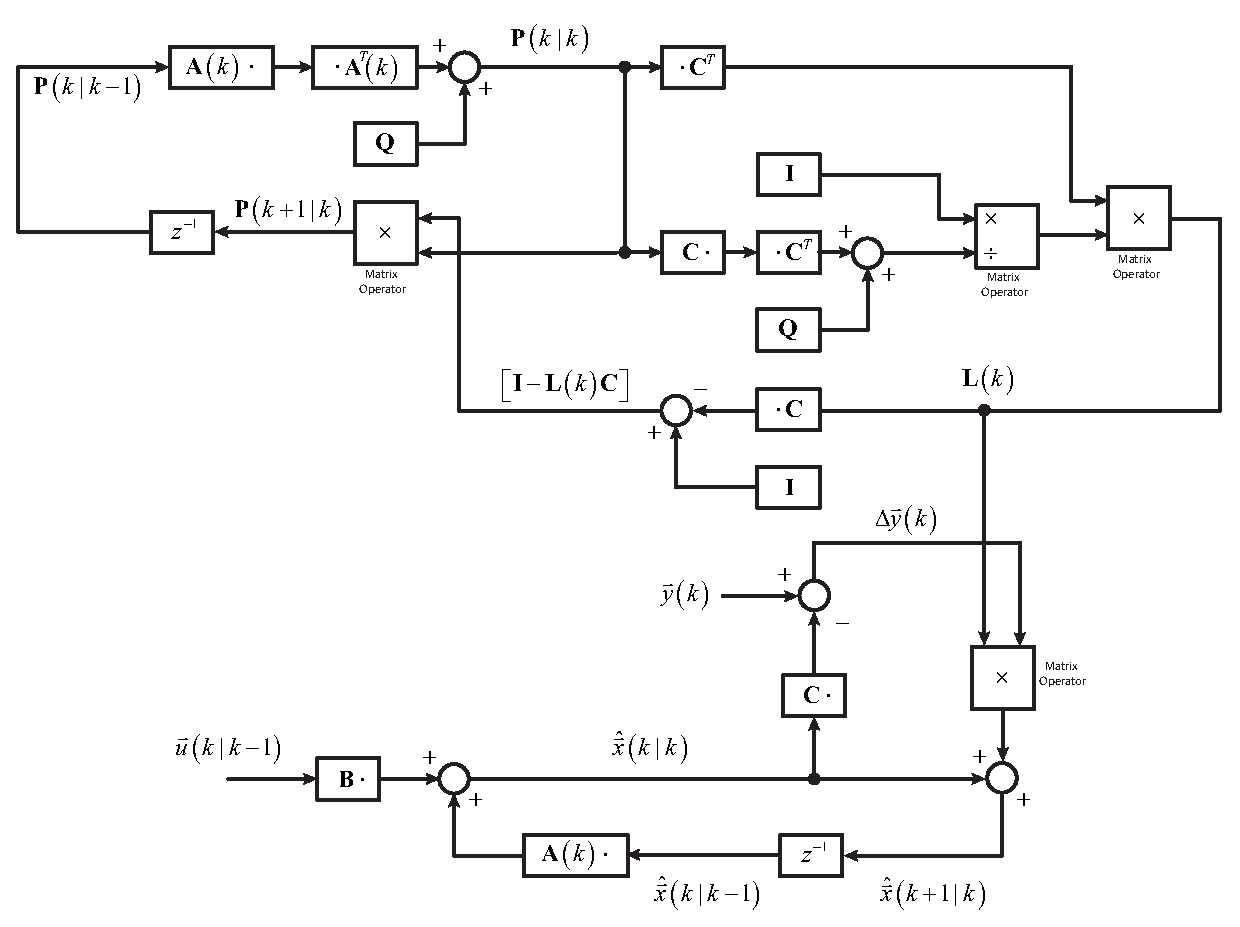
\includegraphics[width = 440pt, angle=0, 
		keepaspectratio]{figures/mpc/kalman_3.eps}
		\captionsetup{width=.5\textwidth}
		\caption{Kalman observer with time varying matrix transition.}
		\label{EKF}
	\end{figure}
\end{mybox}
%\textbf{Discretization.}
%Considering a discretization process at sampling time $t_s$, the equivalent 
%discrete-time model can be approximated as follows:
%\begin{equation}
%	\mathbf{A} = \mathbf{I} + \tilde{\mathbf{A}} \,t_s
%\end{equation}
%\begin{equation}
%	\mathbf{B} = \tilde{\mathbf{B}} \,t_s
%\end{equation}
%\begin{equation*}\label{twophase_ss1d}
%	\left\lbrace \begin{aligned}
	%		{\vec{x}}(k+1) &= {\mathbf{A}}\,\vec{x}(k) + 
	%{\mathbf{B}}\,\vec{u}_{\alpha\beta}(k) \qquad \vec{x}(0) = \begin{bmatrix} 
		%0 & 0 & \Psi^M &  0 \end{bmatrix}^T\\[6pt]
	%		{\vec{y}}(k) &= {\mathbf{C}}\,\vec{x}(k)
	%	\end{aligned}\right. 
%\end{equation*}

\subsection{EKF Observer for nonlinear PMSM}
In additional to the previous EKF observer, we consider now the case where the torque expression is taken into account into the linearization along the observed state trajectory.
\begin{align}\label{}
	\frac{d}{dt}\vec{x}(t)=\vec{g}(\vec{x})\Rightarrow\left\lbrace 
	\begin{aligned}
		\begin{split}
			&\frac{d}{dt}i_\alpha(t) = -\frac{R_s}{L_s}i_\alpha(t) + 	
			\frac{1}{L_s}\omega(t)\psi_\beta^r(t) + \frac{1}{L_s} u_\alpha(t) 
		\end{split}	\\[6pt]
		\begin{split}
			&\frac{d}{dt}i_\beta(t) = -\frac{R_s}{L_s}i_\beta(t) - 	
			\frac{1}{L_s}\omega(t)\psi_\alpha^r(t) + \frac{1}{L_s} u_\beta(t)	
		\end{split}	\\[6pt]
		\begin{split}
			&\frac{d}{dt}\psi_\alpha^r(t) = -\omega(t)\psi_\beta^r(t)
		\end{split}	\\[6pt]
		\begin{split}	
			&\frac{d}{dt}\psi_\beta^r(t) = \omega(t)\psi_\alpha^r(t)	
		\end{split}	\\[6pt]
		\begin{split}
			&\frac{d}{dt}\vartheta(t) = \omega(t)
		\end{split}	\\[6pt]
		\begin{split}
			&\frac{d}{dt}\omega(t) = 
			\frac{p}{J}\Bigg\{\frac{3}{2}p\Big[\psi^r_{\alpha}(t)i_{\beta}(t) - 
			\psi^r_{\beta}(t)i_{\alpha}(t)\Big] - \tau_l(t) 
			-\frac{b}{p}\omega(t)\Bigg\}
		\end{split}
	\end{aligned}\right. 
\end{align}
where we assumed $L_\alpha = \L_\beta = L_s$ and $\frac{1}{p}\omega(t) = \omega_m(t)$.
\begin{mybox}
	\begin{equation}\label{}
		\begin{aligned}
			\left.\frac{\partial}{\partial 
				\vec{x}}\vec{g}(\vec{x})\right|_{\vec{x}=\hat{\vec{x}}} &= 
			\begin{bmatrix} \frac{\partial g_1}{\partial x_1} & \cdots & 
				\frac{\partial g_1}{\partial x_n} \\[6pt]
				\vdots & \ddots & \vdots \\[6pt]
				\frac{\partial g_n}{\partial x_1} & \cdots & \frac{\partial 
					g_n}{\partial x_n}
			\end{bmatrix}_{\hat{\vec{x}}(t)} \\[8pt]
			&= \begin{bmatrix} 
				-\frac{R_s}{L_s} & 0 & 0 & \frac{\hat{\omega}}{L_s} & 0 & \frac{\hat{\psi}_\beta}{L_s} \\[6pt]			
				0 & -\frac{R_s}{L_s} & -\frac{\hat{\omega}}{L_s} & 0 & 0 & -\frac{\hat{\psi}_\alpha}{L_s} \\[6pt]
				0 & 0 & 0 & -\hat{\omega} & 0 & -\hat{\psi}_\beta \\[6pt]
				0 & 0 & \hat{\omega} & 0 & 0 & \hat{\psi}_\alpha \\[6pt]
				0 & 0 & 0 & 0 & 0 & 1 \\[6pt]
				-\frac{3}{2}\frac{p^2}{J}\hat{\psi}_\beta & \frac{3}{2}\frac{p^2}{J}\hat{\psi}_\alpha
				& \frac{3}{2}\frac{p^2}{J}\hat{i}_\beta & -\frac{3}{2}\frac{p^2}{J}\hat{i}_\alpha & 0 & -\frac{b}{J}
			\end{bmatrix}  \\[8pt]
			&=\tilde{\mathbf{A}}_1 + 
			\hat{\omega}(t) \tilde{\mathbf{A}}_2 + \hat{\psi}_\alpha^r(t) 
			\tilde{\mathbf{A}}_3 + \hat{\psi}_\beta^r(t) \tilde{\mathbf{A}}_4
			+ \hat{i}_\alpha(t) 
			\tilde{\mathbf{A}}_5 + \hat{i}_\beta(t) \tilde{\mathbf{A}}_6
		\end{aligned}
	\end{equation} 
	where $\hat{\vec{x}}$ is the estimated state vector from the EKF.
\end{mybox}

The matrices $\tilde{\mathbf{A}}_1$, $\tilde{\mathbf{A}}_2$, 
$\tilde{\mathbf{A}}_3$, $\tilde{\mathbf{A}}_4$, $\tilde{\mathbf{A}}_5$ and $\tilde{\mathbf{A}}_6$ are as follows
\begin{equation}\label{}
	\begin{aligned}
		&\tilde{\mathbf{A}}_1 = 
		\begin{bmatrix} 
			-\frac{R_s}{L_s} & 0 & 0 & 0 & 0 & 0 \\[6pt]			
			0 & -\frac{R_s}{L_s} & 0 & 0 & 0 & 0 \\[6pt]
			0 & 0 & 0 & 0 & 0 & 0 \\[6pt]
			0 & 0 & 0 & 0 & 0 & 0 \\[6pt]
			0 & 0 & 0 & 0 & 0 & 1 \\[6pt]
			0 & 0 & 0 & 0 & 0 & -\frac{b}{J}
		\end{bmatrix},\quad
		\tilde{\mathbf{A}}_2 = 
		\begin{bmatrix} 
			0 & 0 & 0 & \frac{1}{L_s} & 0 & 0 \\[6pt]			
			0 & 0 & -\frac{1}{L_s} & 0 & 0 & 0 \\[6pt]
			0 & 0 & 0 & -1 & 0 & 0 \\[6pt]
			0 & 0 & 1 & 0 & 0 & 0 \\[6pt]
			0 & 0 & 0 & 0 & 0 & 0 \\[6pt]
			0 & 0 & 0 & 0 & 0 & 0
		\end{bmatrix} \\[8pt]
	\end{aligned}
\end{equation}

\begin{equation}
	\begin{aligned}
		&\tilde{\mathbf{A}}_3 = 
		\begin{bmatrix} 
			0 & 0 & 0 & 0 & 0 & 0 \\[6pt]			
			0 & 0 & 0 & 0 & 0 & -\frac{1}{L_s} \\[6pt]
			0 & 0 & 0 & 0 & 0 & 0 \\[6pt]
			0 & 0 & 0 & 0 & 0 & 1 \\[6pt]
			0 & 0 & 0 & 0 & 0 & 0 \\[6pt]
			0 & \frac{3}{2}\frac{p^2}{J} & 0 & 0 & 0 & 0
		\end{bmatrix},\quad
		\tilde{\mathbf{A}}_4 = 
		\begin{bmatrix} 
			0 & 0 & 0 & 0 & 0 & \frac{1}{L_s} \\[6pt]			
			0 & 0 & 0 & 0 & 0 & 0 \\[6pt]
			0 & 0 & 0 & 0 & 0 & -1 \\[6pt]
			0 & 0 & 0 & 0 & 0 & 0 \\[6pt]
			0 & 0 & 0 & 0 & 0 & 0 \\[6pt]
			-\frac{3}{2}\frac{p^2}{J} & 0 & 0 & 0 & 0 & 0
		\end{bmatrix} 
	\end{aligned}
\end{equation} 

\begin{equation}
	\begin{aligned}
		&\tilde{\mathbf{A}}_5 = 
		\begin{bmatrix} 
			0 & 0 & 0 & 0 & 0 & 0 \\[6pt]			
			0 & 0 & 0 & 0 & 0 & 0 \\[6pt]
			0 & 0 & 0 & 0 & 0 & 0 \\[6pt]
			0 & 0 & 0 & 0 & 0 & 0 \\[6pt]
			0 & 0 & 0 & 0 & 0 & 0 \\[6pt]
			0 & 0 & 0 & -\frac{3}{2}\frac{p^2}{J} & 0 & 0
		\end{bmatrix},\quad
		\tilde{\mathbf{A}}_6 = 
		\begin{bmatrix} 
			0 & 0 & 0 & 0 & 0 & 0 \\[6pt]			
			0 & 0 & 0 & 0 & 0 & 0 \\[6pt]
			0 & 0 & 0 & 0 & 0 & 0 \\[6pt]
			0 & 0 & 0 & 0 & 0 & 0 \\[6pt]
			0 & 0 & 0 & 0 & 0 & 0 \\[6pt]
			0 & 0 & \frac{3}{2}\frac{p^2}{J} & 0 & 0 & 0
		\end{bmatrix} 
	\end{aligned}
\end{equation} 
The discretization of the transition matrix $\tilde{\mathbf{A}}(t)$ can be 
approximated by Taylor as follows
\begin{equation}\label{}
	\begin{aligned}
		{\mathbf{A}}(k|k-1) &= \mathbf{I}_6 + \tilde{\mathbf{A}}_1t_s + 
		\hat{\omega}(k|k-1) \tilde{\mathbf{A}}_2t_s +\\[8pt]
		&\quad + \hat{\psi}_\alpha^r(k|k-1) \tilde{\mathbf{A}}_3t_s  + \hat{\psi}_\beta^r(k|k-1) \tilde{\mathbf{A}}_4t_s +\\[8pt]
		&\quad + \hat{i}_\alpha(k|k-1) \tilde{\mathbf{A}}_5t_s + \hat{i}_\beta(k|k-1) \tilde{\mathbf{A}}_6t_s.
	\end{aligned}
\end{equation}

\subsection{Space Vector (SV) and Model Predictive (MP) Modulators}	
In this section a brief overview of the space vector modulation (\textit{SVM}) is reported.  Figure~\ref{space_vector_1} depicts the voltages which a three phase inverter can actuate as function of the switches state in $\alpha\beta$ fixed reference frame representation.

Figure~\ref{space_vector_1b} shows an example of a generic voltage actuation using a combination of adjacent state voltage vectors. The space vector hexagon can be divided into six sectors. For a given output voltage, the corresponding sector have to be identified. Once the sector is identified the ``realization'' of the output vector is made by a time combination of the adjacent three space vector voltages ($\vec{v}_n$, $\vec{v}_{n+1}$, and $\vec{v}_0$).
\begin{figure}[H]
	\centering
	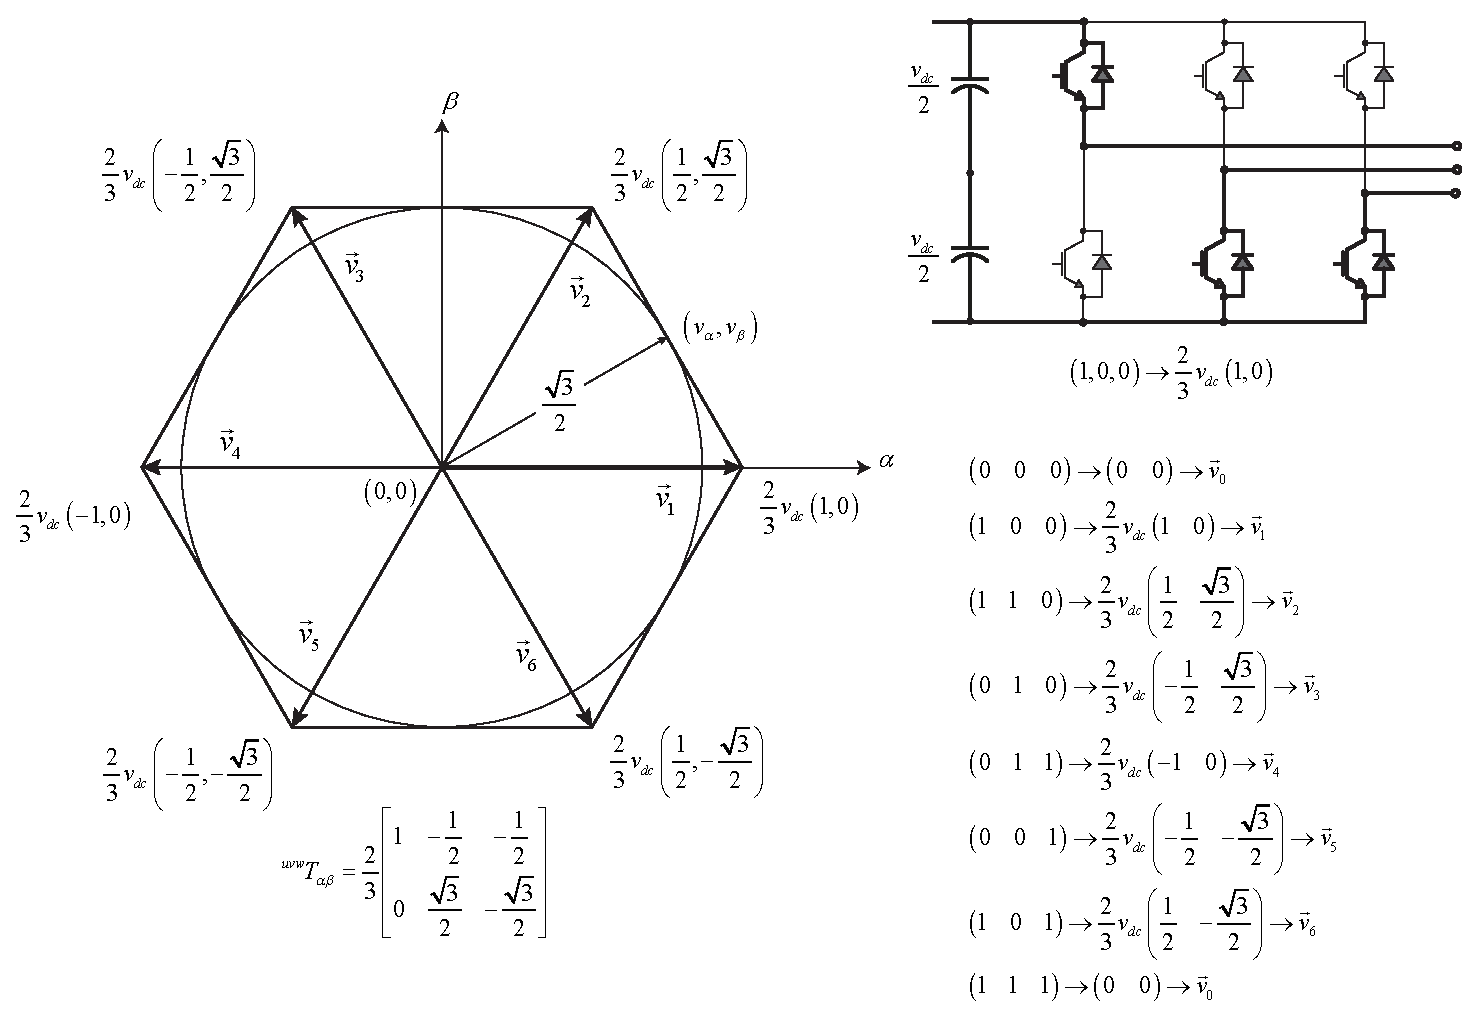
\includegraphics[width = 475pt, angle = 0, 
	keepaspectratio]{figures/vector_modulator/space_vector_1.eps}
	\captionsetup{width=0.5\textwidth, font=small}	
	\caption{Representation of the space vector modulation and relation with inverter switches state.}
	\label{space_vector_1}
\end{figure}
\begin{figure}[H]
	\centering
	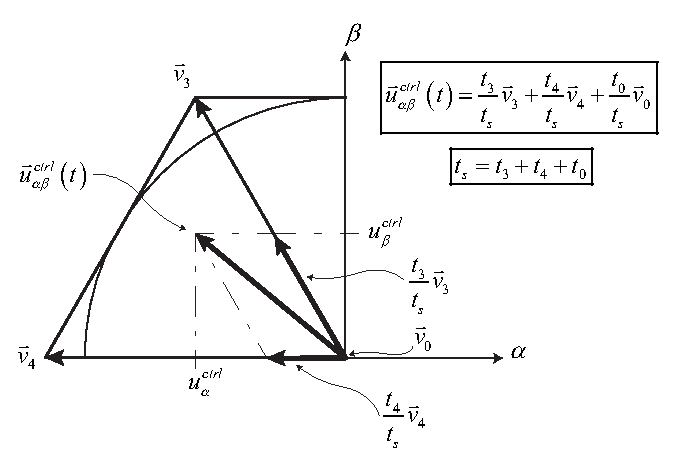
\includegraphics[width = 300pt, angle = 0, 
	keepaspectratio]{figures/vector_modulator/space_vector_1c.eps}
	\captionsetup{width=0.5\textwidth, font=small}	
	\caption{Space vector representation of a generic voltage vector $\vec{u}_{\alpha\beta}$.}
	\label{space_vector_1b}
\end{figure}
Define $t_s$ the switching period of the \textit{SVM}, any vector $\vec{v}_{\alpha\beta}$ (in some case the notation $\vec{v}_{\xi\eta}$ is used) located in the sector $n$ of the space vector hexagon can be ``realized'' by the time combination of the adjacent vectors ($\vec{v}_n$, $\vec{v}_{n+1}$, and $\vec{v}_0$), as follows
\begin{flalign}
	\vec{v}_{\alpha\beta} = \frac{t_n}{t_s}\vec{v}_n + \frac{t_{n+1}}{t_s}\vec{v}_{n+1} + \frac{t_0}{t_s}\vec{v}_0
\end{flalign} 
where $t_n+t_{n+1}+t_0 = t_s$.

In Figure~\ref{space_vector_23}--Figure~\ref{space_vector_89} the relation between the state of the inverter switching bridge and the space voltage vector representation in $\alpha\beta$ is depicted.
\begin{figure}[H]
	\centering
	\begin{subfigure}{0.5\textwidth}
		\centering
		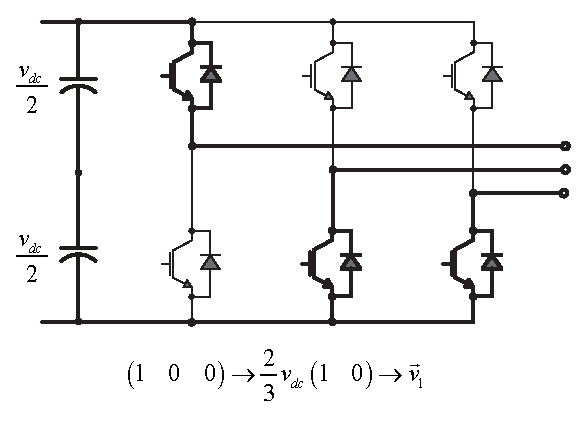
\includegraphics[width = 200pt, angle = 0, 
		keepaspectratio]{figures/vector_modulator/space_vector_2.eps}
		\captionsetup{width=0.45\textwidth, font=footnotesize}	
		\caption{Voltage vector $v_1$ representation.}
		\label{space_vector_2}
	\end{subfigure}%
	\begin{subfigure}{0.5\textwidth}
		\centering
		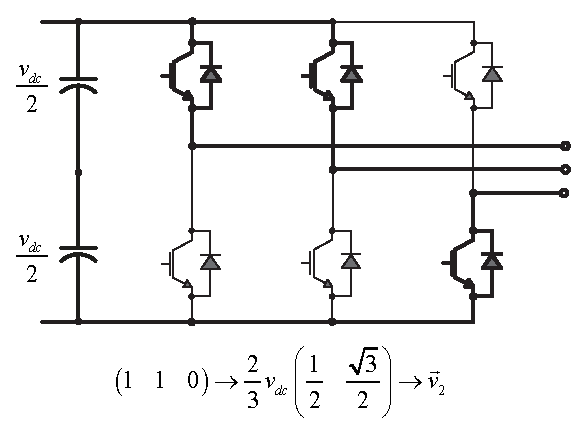
\includegraphics[width = 200pt, angle = 0, 
		keepaspectratio]{figures/vector_modulator/space_vector_3.eps}
		\captionsetup{width=0.45\textwidth, font=footnotesize}	
		\caption{Voltage vector $v_2$ representation.}
		\label{space_vector_3}
	\end{subfigure}
	\captionsetup{width=0.5\textwidth, font=small}	
	\caption{Inverter state representation of the voltages $v_1$ and $v_2$.}
	\label{space_vector_23}
\end{figure}
\begin{figure}[H]
	\centering
	\begin{subfigure}{0.5\textwidth}
		\centering
		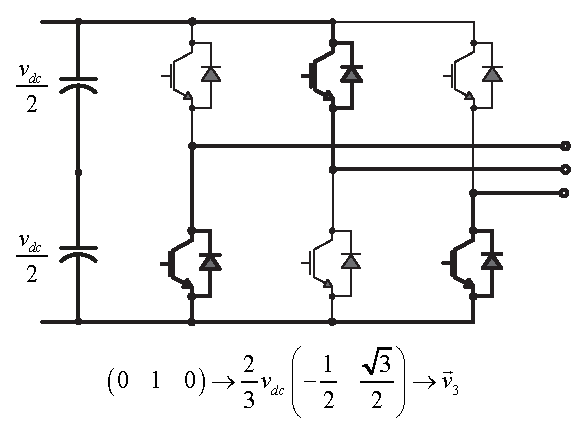
\includegraphics[width = 200pt, angle = 0, 
		keepaspectratio]{figures/vector_modulator/space_vector_4.eps}
		\captionsetup{width=0.45\textwidth, font=footnotesize}	
		\caption{Voltage vector $v_3$ representation.}
		\label{space_vector_4}
	\end{subfigure}%
	\begin{subfigure}{0.5\textwidth}
		\centering
		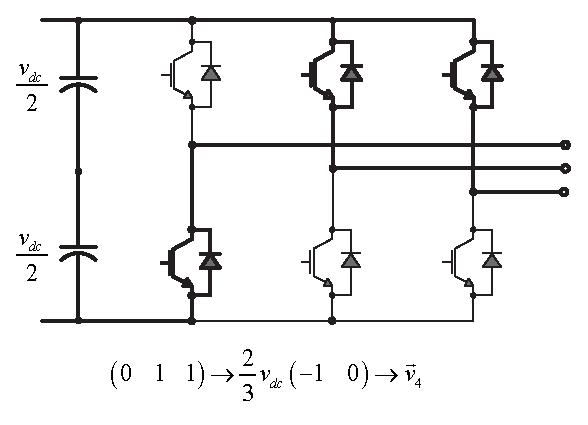
\includegraphics[width = 200pt, angle = 0, 
		keepaspectratio]{figures/vector_modulator/space_vector_5.eps}
		\captionsetup{width=0.45\textwidth, font=footnotesize}	
		\caption{Voltage vector $v_4$ representation.}
		\label{space_vector_5}
	\end{subfigure}
	\captionsetup{width=0.5\textwidth, font=small}	
	\caption{Inverter state representation of the voltages $v_3$ and $v_4$.}
	\label{space_vector_45}
\end{figure}
\begin{figure}[H]
	\centering
	\begin{subfigure}{0.5\textwidth}
		\centering
		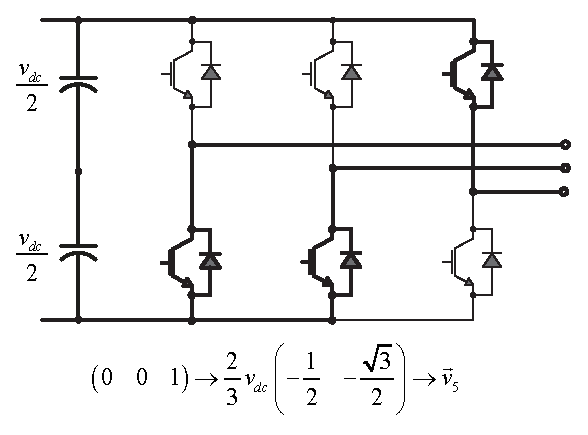
\includegraphics[width = 200pt, angle = 0, 
		keepaspectratio]{figures/vector_modulator/space_vector_6.eps}
		\captionsetup{width=0.45\textwidth, font=footnotesize}	
		\caption{Voltage vector $v_5$ representation.}
		\label{space_vector_6}
	\end{subfigure}%
	\begin{subfigure}{0.5\textwidth}
		\centering
		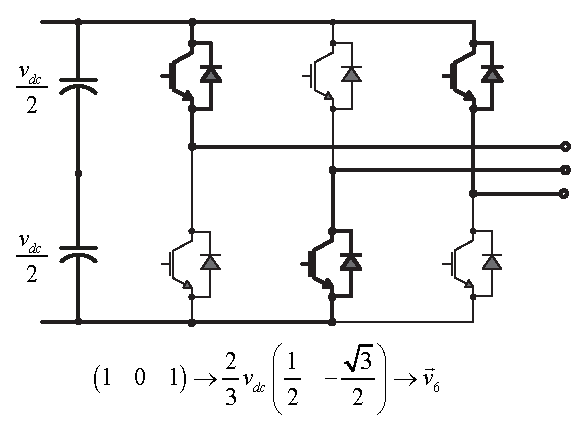
\includegraphics[width = 200pt, angle = 0, 
		keepaspectratio]{figures/vector_modulator/space_vector_7.eps}
		\captionsetup{width=0.45\textwidth, font=footnotesize}	
		\caption{Voltage vector $v_6$ representation.}
		\label{space_vector_7}
	\end{subfigure}
	\captionsetup{width=0.5\textwidth, font=small}	
	\caption{Inverter state representation of the voltages $v_5$ and $v_6$.}
	\label{space_vector_67}
\end{figure}
\begin{figure}[H]
	\centering
	\begin{subfigure}{0.5\textwidth}
		\centering
		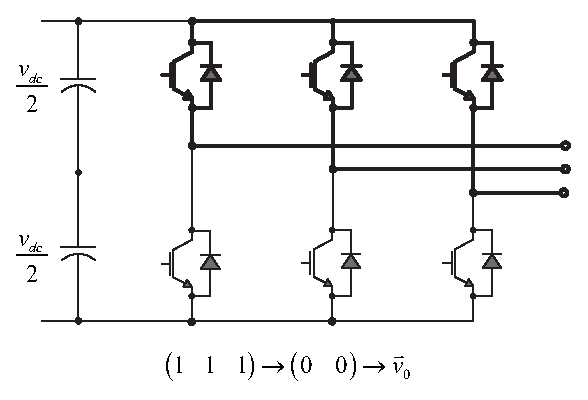
\includegraphics[width = 200pt, angle = 0, 
		keepaspectratio]{figures/vector_modulator/space_vector_8.eps}
		\captionsetup{width=0.45\textwidth, font=footnotesize}	
		\caption{Voltage vector $v_0$ representation - case 1.}
		\label{space_vector_8}
	\end{subfigure}%
	\begin{subfigure}{0.5\textwidth}
		\centering
		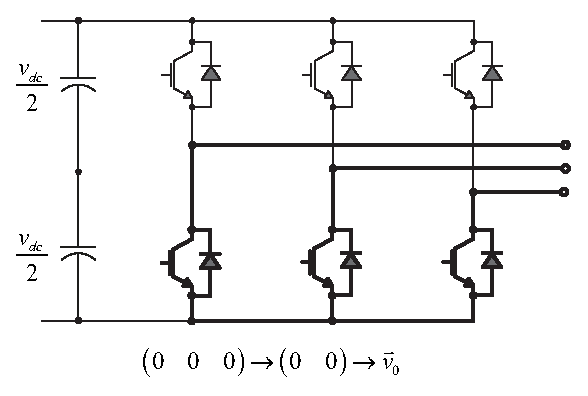
\includegraphics[width = 200pt, angle = 0, 
		keepaspectratio]{figures/vector_modulator/space_vector_9.eps}
		\captionsetup{width=0.45\textwidth, font=footnotesize}	
		\caption{Voltage vector $v_0$ representation - case 2.}
		\label{space_vector_9}
	\end{subfigure}
	\captionsetup{width=0.5\textwidth, font=small}	
	\caption{Inverter state representations of the voltage $v_0$.}
	\label{space_vector_89}
\end{figure}


Concerning the MP-control implementation it is necessary to identity all 
possible $\Big(u_\alpha(k),\ u_\beta(k)\Big)$ output voltage and also define 
the constraint. For a given couple of components $\Big(u_\alpha(k-1),\ 
u_\beta(k-1)\Big)$ exist a finite possible set $\mathcal{U}(k)$ of 
$\Big(u_\alpha(k),\ u_\beta(k)\Big)$ components as shown in the 
Table~\ref{mpc_sv_map}

\begin{table}[H]
	\small
	\begin{center}
		\begin{tblr}{
				hlines,
				vlines,
				row{1}={bg=lightgray}
			} 
			$\Big(u_\alpha(k-1),\ u_\beta(k-1)\Big)\quad$ & $\quad 
			\mathcal{U}(k)$	\\
			$\big(0,\,0\big)\quad$ & $\quad\frac{2}{3}\left\lbrace 
			\big(0,\,0\big);\,\big(1,\,0\big);\,\big(\frac{1}{2},\, \frac{\sqrt{3}}{2} 
			\big);\,\big(-\frac{1}{2},\,\frac{\sqrt{3}}{2}\big); 
			\,\big(-1,\,0\big);\,\big(-\frac{1}{2},\, 
			-\frac{\sqrt{3}}{2}\big);\,\big(\frac{1}{2},\, 
			-\frac{\sqrt{3}}{2}\big)\right\rbrace$ 	\\
			$\frac{2}{3}\big(1,\,0\big)\quad$&$\quad\frac{2}{3}\left\lbrace 
			\big(0,\,0\big);\,\big(1,\,0\big);\,\big(\frac{1}{2},\, 
			\frac{\sqrt{3}}{2}\big);\,\big(\frac{1}{2},\,- 
			\frac{\sqrt{3}}{2}\big)\right\rbrace$	\\
			$\frac{2}{3}\big(\frac{1}{2},\,\frac{\sqrt{3}}{2} 
			\big)\quad$&$\quad\frac{2}{3}\left\lbrace
			\big(0,\,0\big);\,\,\big(\frac{1}{2},\,\frac{\sqrt{3}}{2} 
			\big);\,\big(1,\,0\big);\,\big(-\frac{1}{2},\, 
			\frac{\sqrt{3}}{2}\big)\right\rbrace$ 	\\
			$\frac{2}{3}\big(-\frac{1}{2},\,\frac{\sqrt{3}}{2}\big) 
			\quad$&$\quad\frac{2}{3}\left\lbrace
			\big(0,\,0\big);\,\,\big(-\frac{1}{2},\,\frac{\sqrt{3}}{2}\big);\, 
			\big(-1,\,0\big);\,\big(\frac{1}{2},\,\frac{\sqrt{3}}{2}\big)\right\rbrace$ \\
			$\frac{2}{3}\big(-1,\,0\big)\quad$&$\quad\frac{2}{3}\left\lbrace 
			\big(0,\,0\big);\,\big(-1,\,0\big);\,\big(-\frac{1}{2},\, 
			\frac{\sqrt{3}}{2}\big);\,\big(-\frac{1}{2},\, 
			-\frac{\sqrt{3}}{2}\big)\right\rbrace$	\\
			$\frac{2}{3}\big(-\frac{1}{2},\,-\frac{\sqrt{3}}{2}\big) 
			\quad$&$\quad\frac{2}{3}\left\lbrace
			\big(0,\,0\big);\,\,\big(-\frac{1}{2},\,-\frac{\sqrt{3}}{2}\big);\, 
			\big(-1,\,0\big);\,\big(\frac{1}{2},\,\frac{\sqrt{3}}{2}\big)\right\rbrace$ \\
			$\frac{2}{3}\big(\frac{1}{2},\,-\frac{\sqrt{3}}{2}\big) 
			\quad$&$\quad\frac{2}{3}\left\lbrace
			\big(0,\,0\big);\,\,\big(\frac{1}{2},\,-\frac{\sqrt{3}}{2}\big);\, 
			\big(1,\,0\big);\,\big(-\frac{1}{2},\,-\frac{\sqrt{3}}{2}\big)\right\rbrace$ \\
		\end{tblr}
	\end{center}
	\captionsetup{width=.5\textwidth}
	\caption{Set of admissible output voltage $\mathcal{U}(k)$ from a given 
		voltage vector $\big(u_\alpha\ u_\beta\big)$.}
	\label{mpc_sv_map}
\end{table}
The knowledge of the space vector commutation law and in particular the knowledge of the set $\mathcal{U}(k)$ because it will affect the implementation of the MPC.


\subsection{Current Reference Generator}
In this subsection we derive the relation between the electromagnetic torque which per PMSM has to provide and the stator current. Basically we will derive the set of current reference
\begin{equation}\label{pmsm_problem_1_eq_17}
	\tau_m^{ref}\rightarrow \big(i_\alpha^{ref},\ i_\beta^{ref}\big)
\end{equation}
where $\tau_m^{ref}$ is the output of the speed control.

As shown in a previous section the electromagnetic torque can be expressed as 
follows
\begin{equation}\label{pmsm_problem_1_eq_18}
	\begin{aligned}
		\tau_m = \frac{3}{2}p\left( 
		\psi^r_{\alpha}i_{\beta}-\psi^r_{\beta}i_{\alpha}\right) 
	\end{aligned} 
\end{equation}
where $\vec{\psi}^r_{\alpha\beta} = \begin{bmatrix} \Psi^M\cos(\vartheta) &  
	\Psi^M\sin(\vartheta)\end{bmatrix}^T$ are permanent magnet rotor fluxes linkage to the stator, and $p$ the number of pole pairs.

Let $\hat{\vartheta}$ be the estimation of the magnetic flux phase resulted 
from the Kalman observer 
\begin{equation}\label{pmsm_problem_1_eq_19}
	\begin{aligned}
		\hat{\vartheta} = 
		\arctan\left(\hat{\psi}^r_{\beta},\hat{\psi}^r_{\alpha} \right)  
	\end{aligned} 
\end{equation}
That means to achieve the \textit{maximum torque per ampere} we have to build a 
current reference as follows 
\begin{equation}\label{pmsm_problem_1_eq_20}
	\begin{aligned}
		&i_{\alpha}^{ref} = -i^{ref}\sin(\hat{\theta})  \\[6pt]
		&i_{\beta}^{ref} = i^{ref}\cos(\hat{\theta})
	\end{aligned} 
\end{equation}
when $\vartheta - \hat{\vartheta} \rightarrow 0$ the applied torque results in
\begin{equation}\label{pmsm_problem_1_eq_21}
	\begin{aligned}
		\tau_m &= \frac{3}{2}p\left( 
		\psi^r_{\alpha}i_{\beta}-\psi^r_{\beta}i_{\alpha}\right) \\[6pt]
		&= \begin{bmatrix}
			i_{\alpha} & i_{\beta}
		\end{bmatrix} \begin{bmatrix}
			0 & -1 \\[6pt] 1 & 0
		\end{bmatrix}\begin{bmatrix}
			\psi^r_{\alpha} \\[6pt] \psi^r_{\beta}
		\end{bmatrix}\\[6pt]
		&= \begin{bmatrix}
			-i^{ref}\sin(\hat{\theta}) & i^{ref}\cos(\hat{\theta})
		\end{bmatrix} \begin{bmatrix}
			0 & -1 \\[6pt] 1 & 0
		\end{bmatrix}\begin{bmatrix}
			\Psi^M\cos(\vartheta) \\[6pt] \Psi^M\sin(\vartheta)
		\end{bmatrix}\\[6pt]
		&= \frac{3}{2}p\,\Psi^M\,i^{ref} \quad\Leftarrow\vartheta - \hat{\vartheta} \rightarrow 0
	\end{aligned}
\end{equation}
Eq.~\eqref{pmsm_problem_1_eq_21} requires that $\vartheta - \hat{\vartheta} \rightarrow 0$ that means the EKF performance plays a fundamental role in the capability of the overall system to deliver the required amount of electromagnetic torque. 

\subsection{MPC with EKF Implementation}
Up to now we have defined the following substructure
\begin{itemize}
	\item[--] Fluxes observer based on EKF 
	\item[--] Voltge space vector elements available using the two level Inverter.
\end{itemize}
what is missing are 
\begin{itemize}
	\item[--] PI-based speed control, seen in example~\ref{PIDinDTD}
	\item[--] Double Integrator Observer, seen in example~\ref{DoubleIntegratorObserver}
	\item[--] Model predictive control.
\end{itemize}
Let's now going to derive the MPC for the isotropic PMSM.

From the discrete time model of the PMSM described by Eq.~\eqref{pmsm_problem_1_eq_4} we take the first two Kirchhoff's voltage law equations that describe the dynamic of the stator current. 

These two equation will be used to implement our current control based on model predictive. As from hypothesis we assume $L_\alpha=L_\beta=L_s$ which results in
\begin{equation}\label{pmsm_problem_1_eq_22}
	\left\lbrace \begin{aligned}
		&i_\alpha(k+1)=\Big(1-t_s\frac{R_s}{L_s}\Big)i_\alpha(k) + 
		t_s\frac{\hat{\omega}(k)}{L_s}\hat{\psi}_\beta(k) + 
		t_s\frac{1}{L_s}u_\alpha(k) \\[6pt] 
		&i_\beta(k+1)=\Big(1-t_s\frac{R_s}{L_s}\Big)i_\beta(k) - 
		t_s\frac{\hat{\omega}(k)}{L_s}\hat{\psi}_\alpha(k) + 
		t_s\frac{1}{L_s}u_\beta(k)
	\end{aligned}\right. 
\end{equation}
\textbf{These two equations allow predictions of the stator currents to be calculated for 
	each one of the seven voltage vectors generated by the inverter.}

In order to implement a tracking control problem we can assume the following cost function:
\begin{equation}
	g=\Big[i_\alpha^{ref}(k) - i_\alpha^{\mathbf{P}}(k+1)\Big]^2+ 
	\Big[i_\beta^{ref}(k) -i_\beta^{\mathbf{P}}(k+1)\Big]^2
\end{equation}
The MPC algorithm can be summarized as follows
\begin{itemize}
	\item[--] At every step the control determine in which output voltage sector is currently located. 
	\item[--] By the knowledge of the voltage sector the algorithm calculate all current prediction using all possible output voltage which can be actuated from the given voltage sector.
	\item[--] By the knowledge of all current prediction we calculate the value of the cost function for each of all current prediction.
	\item[--] By the knowledge of the cost function value for each current prediction the control determine the value of output voltage for which the cost function is minimal.
	\item[--] The set of output voltage which minimize the cost function will be actuated at the next step.
\end{itemize}

\subsubsection{MPC algorithm implementation}
The control scheme for field oriented control (FOC) of the PMSM using 
predictive current control is shown in Figure~\ref{pmsmctrl}. Here, a PI 
controller is used for the speed control which its output generates the current 
reference according to Eqs.~\ref{speed_conrol_pmsm_eq1}. 
\begin{equation}\label{speed_conrol_pmsm_eq1}
	\frac{d}{dt}{\omega}_m(t) = 
	\frac{1}{J}\tau_m^{ref}(t)
	-\tau_l(t) -b{\omega}_m(t)\Bigg]
\end{equation}
which in terms of current reference
\begin{equation}\label{speed_conrol_pmsm_eq2}
	\frac{d}{dt}{\omega}_m(t) = 
	\frac{1}{J}\Bigg[\frac{3}{2}p\Big[\psi^r_{\alpha}(t)i_{\beta}^{ref}(t)-\psi^r_{\beta}(t)i_{\alpha}^{ref}(t)\Big]
	-\tau_l(t) -b{\omega}_m(t)\Bigg]
\end{equation}
which results in
\begin{equation}\label{speed_conrol_pmsm_eq3}
	\begin{aligned}
		&i_{\alpha}^{ref} = -i^{ref}\sin(\hat{\theta})  \\[6pt]
		&i_{\beta}^{ref} = i^{ref}\cos(\hat{\theta})
	\end{aligned} 
\end{equation}
that means exist and algebraic correlation between 
\begin{equation}
	\tau_m^{ref}(t)=\frac{3}{2}\,p\,\Psi^Mi^{ref}(t)
\end{equation}
where $\tau_m^{ref}(t)$ is the output of the speed control block.

A model predictive controller is used for the current control block. In the 
predictive scheme, the discrete-time model  of the machine is used for 
predicting the stator current components for each seven different voltage 
vectors generated by the inverter. The voltage vector that minimizes a given 
cost function is selected and applied during a whole sampling interval.
The whole motor control scheme is shown in Figure~\ref{pmsmctrl}
\begin{figure}[H]
	\centering
	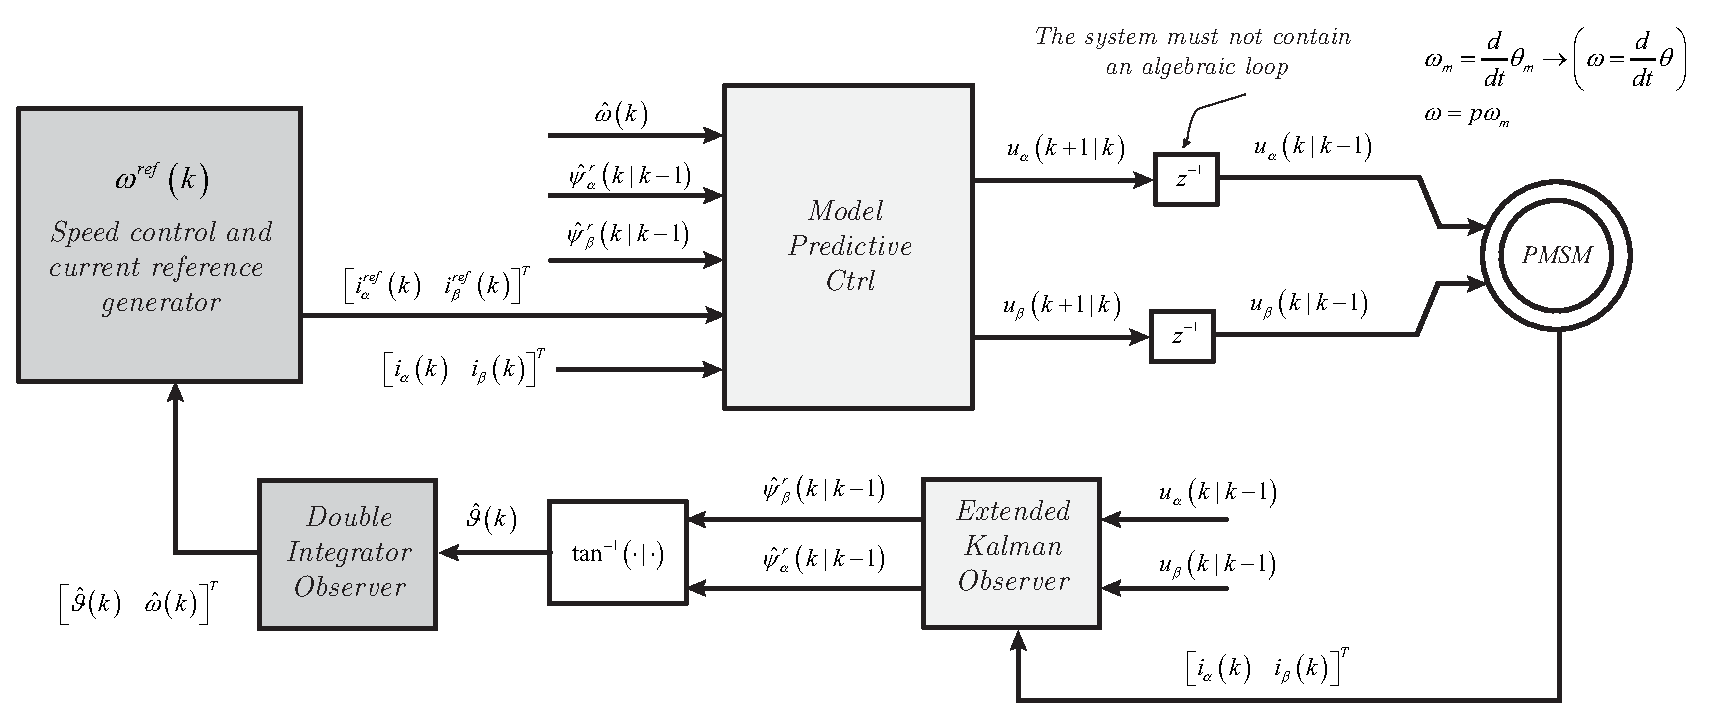
\includegraphics[width = 500pt, angle=0, 
	keepaspectratio]{figures/mpc/pmsm_ctrl_ab_2.eps}
	\captionsetup{width=.5\textwidth}
	\caption{PMSM control architecture.}
	\label{pmsmctrl}
\end{figure}


\subsection{Simulation Results}
Simulation result are here reported. At time ($t=\SI{15}{\second}$) the 
$\psi^M$ permanent magnet flux is slowly reduced (as effect of the increasing 
temperature). An external load is applied as shown in 
Figure~\ref{speed_tracking_pmsm}.
Simulation results for 
\begin{equation}
	\mathbf{Q}=\begin{bmatrix}
		\frac{R_s}{L_s}t_s & 0 & 0 & 0 & 0 & 0 \\ 0 & \frac{R_s}{L_s}t_s & 0 & 
		0 & 0 & 0 \\
		0 & 0 & 2t_s^2 & 0 & 0 & 0 \\ 0 & 0 & 0 & 2t_s^2 & 0 & 0 \\
		0 & 0 & 0 & 0 & t_s & 0 \\ 0 & 0 & 0 & 0 & 0 & t_s \\
	\end{bmatrix} \qquad \mathbf{R}=\begin{bmatrix}
		1 & 0 \\ 0 & 1
	\end{bmatrix}
\end{equation}

\begin{figure}[H]
	\centering
	\begin{subfigure}{.5\textwidth}
		\centering
		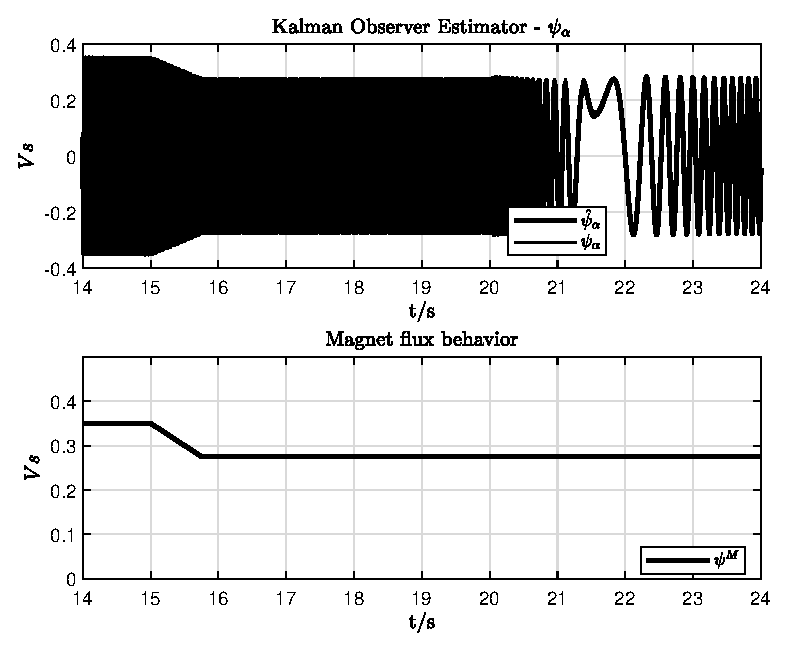
\includegraphics[width = 225pt, angle=0, 
		keepaspectratio]{figures/mpc/observerPSIa.eps}
		\captionsetup{width=.5\textwidth}
		\caption{$\hat{\psi}_\alpha$ flux estimation..}
		\label{}
	\end{subfigure}%
	\begin{subfigure}{.5\textwidth}
		\centering
		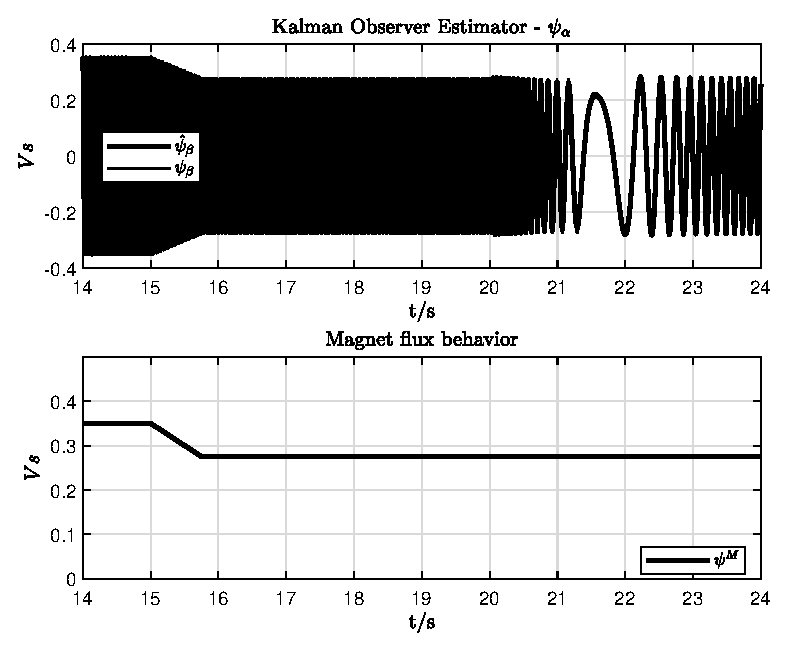
\includegraphics[width = 225pt, angle=0, 
		keepaspectratio]{figures/mpc/observerPSIb.eps}
		\captionsetup{width=.5\textwidth}
		\caption{$\hat{\psi}_\beta$ flux estimation..}
		\label{}
	\end{subfigure}
	\caption{Simulation results.}
	\label{}
\end{figure}
\begin{figure}[H]
	\centering
	\begin{subfigure}{.5\textwidth}
		\centering
		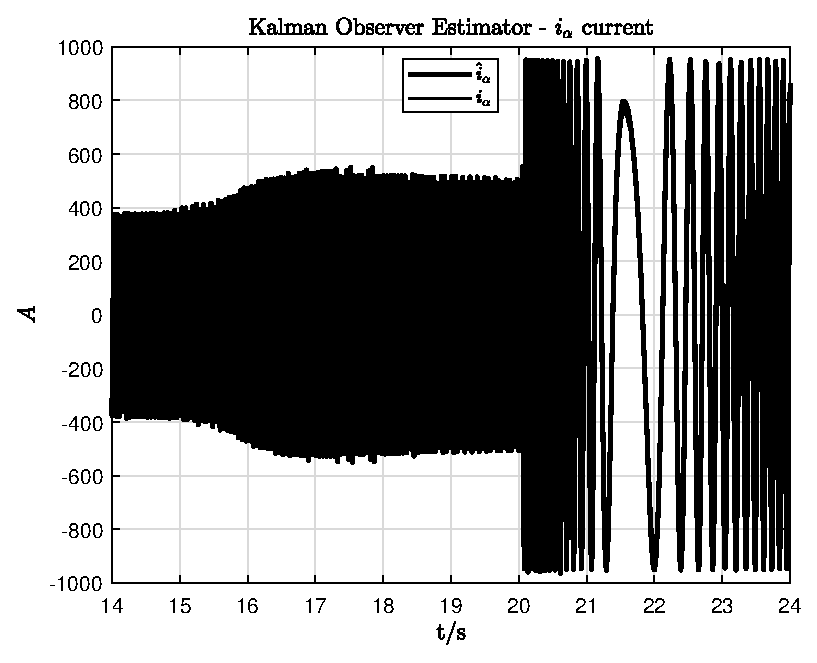
\includegraphics[width = 225pt, angle=0, 
		keepaspectratio]{figures/mpc/observerIa.eps}
		\caption{$\hat{i}_\alpha$ current estimation.}
		\label{}
	\end{subfigure}%
	\begin{subfigure}{.5\textwidth}
		\centering
		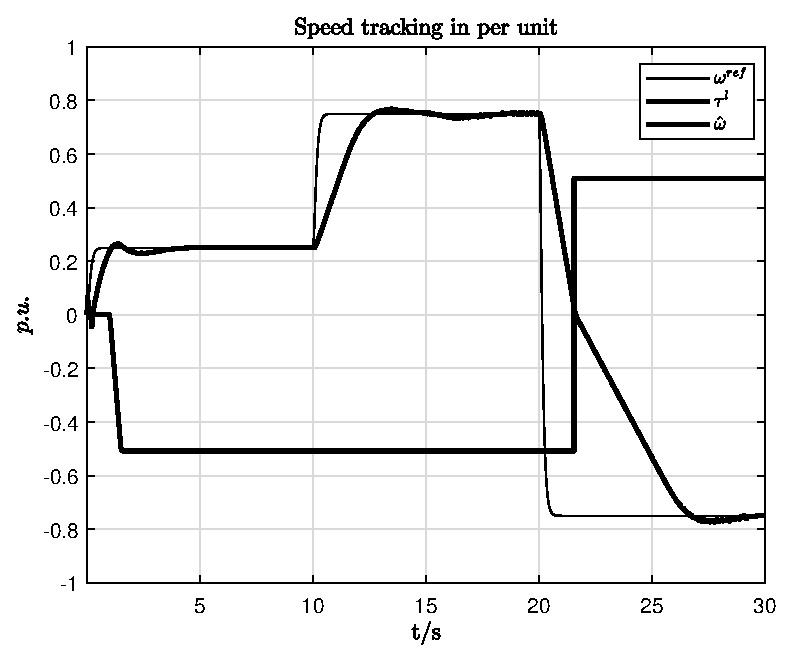
\includegraphics[width = 225pt, angle=0, 
		keepaspectratio]{figures/mpc/SpeedTracking.eps}
		\caption{Speed tracking performance.}
		\label{speed_tracking_pmsm}
	\end{subfigure}
	\caption{Simulation results.}
	\label{}
\end{figure}

\end{onehalfspace}
\end{document} 